\documentclass[]{llncs}
% TODO: get rid of page numbers
\pagestyle{plain}

\usepackage[utf8]{inputenc}
\usepackage{url}
\usepackage{amsmath}
\usepackage{mathbbol}
\usepackage{mathtools}
\usepackage{hyperref}
\usepackage{todonotes}
\usepackage{appendix}

% Two column itemize
\usepackage{multicol}

% Example code
\usepackage{listings}

% Diagrams
\usepackage{tikz}

% Mathbb doesn't support digits
\usepackage{bbm}

% inference rules
\usepackage{mathpartir}

% Newline inside table
\usepackage{makecell}

% Continue examples later on
% \usepackage{thmtools}
% \renewcommand\thmcontinues[1]{Continued}

% Do not use italics in definitions and theorems
\spnewtheorem{nidefinition}[definition]{Definition}{}{}
\spnewtheorem{nilemma}[lemma]{Lemma}{\bfseries}{}
\spnewtheorem{nitheorem}[theorem]{Theorem}{\bfseries}{}

\renewcommand{\sectionautorefname}{\S}%
\renewcommand{\subsectionautorefname}{\S}%
\renewcommand{\appendixautorefname}{Appendix}

% Abbreviations
\newcommand{\lambdacalc}{$\lambda$-calculus}
\newcommand{\picalc}{$\pi$-calculus}
\newcommand{\Picalc}{$\pi$-Calculus}

% Typing rules
\newcommand{\stacked}[1]{\mprset{flushleft} \inferrule*{}{#1}}
\newcommand{\datatype}[2]{{\mprset{fraction={===}} \inferrule{#1}{#2}}}

\newcommand{\type}[1]{\textcolor{blue}{\operatorname{#1}}}
\newcommand{\constr}[1]{\textcolor{orange}{\operatorname{#1}}}
\newcommand{\func}[1]{\textcolor{teal}{\operatorname{#1}}}

% Constructors
\newcommand{\PO}{\constr{\mathbb{0}}}
\newcommand{\comp}[2]{#1 \, \constr{\parallel} \, #2}
\newcommand{\new}{\constr{\boldsymbol{\nu}} \,}
\newcommand{\send}[2]{#1 \, \constr{\langle} \, #2 \,\constr{\rangle} \,}
\newcommand{\recv}[2]{#1 \, \constr{\mathbb{(}} \, #2 \, \constr{\mathbb{)}} \,}
\newcommand{\suc}{\constr{\scriptstyle 1+}}
\newcommand{\unit}{\constr{\mathbbm{1}}}
\newcommand{\base}[1]{\constr{B[} \, #1 \, \constr{]}}
\newcommand{\channel}[2]{\constr{C[} \, #1 \, \constr{;} \, #2 \, \constr{]}}
\newcommand{\comma}{\, \constr{,} \,}

% Functions
\newcommand{\subst}[3]{#1 \, \func{[} \, #3 \, \func{\mapsto} \,#2 \, \func{]}}
\newcommand{\op}[3]{#1 \, \func{\coloneqq} \, #2 \, \func{\cdot} \, #3}
\newcommand{\opsquared}[3]{#1 \, \func{\coloneqq} \, #2 \, \func{\cdot^2} \, #3}
\newcommand{\opctx}[3]{#1 \, \func{\coloneqq} \, #2 \, \func{\otimes} \, #3}
\newcommand{\zero}{\func{0\cdot}}
\newcommand{\one}{\func{1\cdot}}
\newcommand{\li}{\func{\ell_i}}
\newcommand{\lo}{\func{\ell_o}}
\newcommand{\lz}{\func{\ell_{\varepsilon}}}
\newcommand{\lio}{\func{\ell_{\#}}}

% Types
\newcommand{\Set}{\type{SET}}
\newcommand{\reduce}[1]{\, \type{\longrightarrow}_{#1} \,}
\newcommand{\types}[4]{#1 \, \type{;} \, #2 \, \type{\vdash} \, #3 \, \type{\triangleright} \, #4}
\newcommand{\contains}[6]{#1 \, \type{;} \, #2 \, \type{\ni}_{#3} \, #4 \, \type{;} \, #5 \, \type{\triangleright} \, #6}
\newcommand{\containsusage}[4]{#1 \, \type{\ni}_{#2} \, #3 \, \type{\triangleright} \, #4}
\newcommand{\Var}{\type{VAR}}
\newcommand{\Process}{\type{PROCESS}}
\newcommand{\Raw}{\type{RAW}}
\newcommand{\Name}{\type{NAME}}
\newcommand{\Names}{\type{NAMES}}
\newcommand{\Fresh}{\type{FRESH}}
\newcommand{\WellScoped}{\type{WELLSCOPED}}
\newcommand{\Unused}{\type{UNUSED}}
\newcommand{\PreCtx}{\type{PRECTX}}
\newcommand{\Ctx}{\type{CTX}}
\newcommand{\Type}{\type{TYPE}\,}
\newcommand{\Idx}{\type{IDX}\,}
\newcommand{\Idxs}{\type{IDXS}}
\newcommand{\Usage}{\type{USAGE}}
\newcommand{\N}{\type{\mathbb{N}}}
\newcommand{\Channel}{\type{CHANNEL}}
\newcommand{\Rec}{\type{REC}}
\newcommand{\Algebra}{\type{ALGEBRA}}
\newcommand{\eq}{\, \type{\simeq} \,}
\newcommand{\eqeq}{\, \type{\cong} \,}

% Example
\newcommand{\sender}{\textcolor{brown}{sender}}
\newcommand{\receiver}{\textcolor{purple}{receiver}}
\newcommand{\courier}{\textcolor{cyan}{courier}}

%%%%%%%%%%%%%%%%%%%%%%%%%%%%%%%%%%%%%%%%%%%%%%%%%%%%%%%%%%%%%%%%%%%
\title{$\pi$ with leftovers: \\ a mechanisation in Agda}
\titlerunning{$\pi$ with leftovers: a mechanisation in Agda}
\author{
  Uma Zalakain\inst{1}\orcidID{0000-0002-3268-9338}
  \and
  Ornela Dardha\inst{2}\orcidID{0000-0001-9927-7875}
}
\institute{
  University of Glasgow, Scotland \\ \email{u.zalakain.1@research.gla.ac.uk}
  \and
  University of Glasgow, Scotland \\ \email{ornela.dardha@glasgow.ac.uk}
}
% Support
% This work is supported by the UK EPSRC grant EP/K034413/1 ``From Data Types to Session Types: A Basis for Concurrency and Distribution'' (ABCD), and by the EU HORIZON 2020 MSCA RISE project 778233 ``Behavioural Application Program Interfaces'' (BehAPI).}

%%%%%%%%%%%%%%%%%%%%%%%%%%%%%%%%%%%%%%%%%%%%%%%%%%%%%%%%%%%%%%%%%%% 

\begin{document}


\maketitle

\begin{abstract}
  Linear type systems need to keep track of how programs use their resources.
  The standard approach is to use context splits, side conditions that specify how resources are disjointly split across subterms.
  With this approach, context splits echo information which is already present within subterms, thus leading to redundancy.  An alternative approach is to use leftover typing \cite{Mackie,Allais2018a}, where in addition to the usual (input) usage context, typing judgments have an additional output usage context: the leftovers.
  With this approach, the leftovers of one typing derivation can be fed as the inputs of the next, threading through linear resources while avoiding context splits.
  We use this technique to define a type system for a resource-aware \picalc{} \cite{MilnerPW92,Milner99}.
  This type system is parametrised over a set of usage algebras that are general enough to encompass shared types (free to reuse and discard), graded types (use an $n$ number of times) and linear types (use exactly once).
  We provide a framing theorem, generalise the weakening and strengthening theorems, and show subject reduction.
  Our formalisation is fully mechanised in about 1800 lines of Agda.

%  \keywords{Pi-calculus \and Linear types \and Leftover typing \and Concurrency \and Mechanisation \and Agda}
\end{abstract}

%%%%%%%%%%%%%%%%%%%%%%%%%%%%%%%%%%%%%%%%%%%%%%%%%%%%%%%%%%%%%%%%%%%
\section{Introduction}

%Recent years have seen an increase in the efforts to mechanise linear process algebras \cite{Gay2001,Goto2016a,Gay2010,Thiemann2019,Ciccone}
A linear type system guarantees that resources are used \emph{exactly once}.
Enforcing this ``no duplicating'' and ``no discarding'' of resources via linearity allows for resource-aware programming and more efficient implementations \cite{Wadler90}.
Such a linear type system needs to keep track of what resources are used in which parts of the program.
To do so, the standard approach is to use context splits: typing rules for terms with multiple subterms use a side condition that specifies what resources to allocate to each of the subterms.
The typing derivations for the subterms must then use the entirety of the resources allocated to them.
A key observation here is that each subterm already \emph{knows} about the resources it needs.
\emph{Context splits contain usage information already present in the subterms.}
Moreover, the subterms cannot be typed until the context splits have been defined.
On top of that, using binary context splits means that typing rules with $n$ subterms require $n - 1$ context splits, which considerably clutters the type system.

An alternative approach to using context splits is using leftover typing, which has been used to formulate intuitionistic linear logic \cite{Mackie} and to mechanise the linear \lambdacalc \cite{Allais2018a}.

In this paper, we use leftover typing to define a resource-aware type system for the \picalc{}.
The \picalc{} \cite{MilnerPW92,Milner99} is a computational model for communication and concurrency that boils concurrent processing down to the sending and receiving of data over communication channels.
Notably, it features channel mobility: channels themselves are first class values, and can therefore be sent and received.
%Kobayashi et al. \cite{KPT96} introduced a typed version of the \picalc{} where the linear type system restricts the usage of channels to exactly once.

Leftover typing changes the shape of the typing judgments and includes a second \emph{leftover} output context that contains the resources that were not used by the term.
As a result, typing rules \emph{thread the resources through} subterms without needing context splits: each subterm uses the resources it needs, and leaves the rest for its siblings.
The first subterm in this chain of resources immediately knows what resources it has available.
Below we present two alternative typing rules for process composition in the linear \picalc{}: the one on the left uses context splits, while the one on the right uses leftover typing.
\begin{mathpar}
  \inferrule
  {\opctx{\Gamma}{\Delta}{\Xi} \\ \Delta \; \type{\vdash} \; P \\ \Xi \; \type{\vdash} \; Q}
  {\Gamma \; \type{\vdash} \; \comp{P}{Q}}

  \inferrule
  {\Gamma \; \type{\vdash} \; P \; \type{\triangleright} \; \Delta \\ \Delta \; \type{\vdash} \; P \; \type{\triangleright} \; \Xi}
  {\Gamma \; \type{\vdash} \; \comp{P}{Q} \; \type{\triangleright} \; \Xi}
\end{mathpar}

We make the following main contributions in this paper:
\begin{enumerate}
  \item \textbf{Leftover typing for a resource-aware \picalc{}}. Our type system uses leftover typing to model the resource-aware \picalc{} (\autoref{leftover-typing}) and satisfies subject reduction.
    In addition to making context splits unnecessary, leftover typing allows for a \emph{framing} theorem to be stated and is naturally associative, making type safety properties considerably easier to reason about (\autoref{meta-theory}).
        
  \item \textbf{Shared, graded and linear unified \picalc{}}.
  We {generalise resource counting to a set of usage algebras that can be mixed within the same type system}.
    We do not instantiate our type system to only work with linear resources, instead we present an algebra-agnostic type system, and admit a mix of user-defined \emph{resource aware} algebras (\autoref{multiplicities}).
    Any \emph{partial commutative monoid} that is \emph{decidable}, \emph{deterministic}, \emph{cancellative} and has a \emph{minimal element} is a valid such algebra.
    Multiple algebras can be mixed in the type system --- usage contexts keep information about what algebra to for each type (\autoref{contexts}).
    In particular, this allows for type systems combining linear (use exactly once), graded (exact number of $n$ times) and shared (free to reuse and discard) types under the same framework.
    Thanks to leftovers, our type system satisfies \emph{weakening} and \emph{strengthening} for the whole framework. In particular, these are stated for the first time for the linear \picalc{}.
    
    \item \textbf{Full mechanisation in Agda}. We have fully mechanised a proof of subject reduction, the details of which are found in \autoref{app:type-safety}
The formalisation of the \picalc{} with leftover typing, from the syntax to the semantics and the type system, has been fully mechanised in Agda in about 1850 lines of code, and is publicly available in our GitHub repository \cite{Zalakain2020Agda}.

\end{enumerate}

We start by using type level {de Bruijn indices} \cite{deBruijn1972,Dybjer1994} to introduce a syntax of \picalc{} processes that is \emph{well scoped by construction}: every free variable is accounted for in the type of the process that uses it (\autoref{syntax}).
We then provide an operational semantics for the \picalc{}, prior to any typing (\autoref{semantics}).
This operational semantics is defined as a reduction relation on processes (\autoref{operational-semantics}).
The reduction relation tracks at the type level the channel on which communication occurs.
This information is later used to state the subject reduction theorem --- aka type preservation.
The reduction relation is defined modulo \emph{structural congruence} (\autoref{structural-congruence}) --- a relation defined on processes that acts as a quotient type to remove unnecessary syntactic minutiae introduced by the syntax of the \picalc{}.
We then define an interface for resource-aware algebras (\autoref{multiplicities}) and use it to parametrise a type system based on leftover typing (\autoref{leftover-typing}).
Finally, we present the meta theoretical properties of our \picalc{} with leftovers in \autoref{meta-theory}.

\subsection{Notation}
%%%%%%%%%%%%%%%%%%%%%%%%%%%%%%%%%%%%%%%%%%%%%%%%%%%%%%%%%%%%%%%%%%%

We briefly illustrate the notation used in this paper.
Data type definitions ($\type{\N}$) use double inference lines and index-free synonyms (\textsc{Nat}) as rule names for ease of reference.
Constructors ($\constr{0}$ and $\suc$) are given as inference rules.
We maintain a close correspondence between the definitions presented in this paper and our mechanised definitions in Agda: inference rules become type constructors, premises become argument types and conclusions return types.
Universe levels and universe polymorphism are omitted for brevity --- all our types are of type $\Set$.
Implicit arguments are mentioned in type definitions but omitted by constructors.
\begin{mathpar}
  \datatype
  { }
  {\type{\N} : \Set}
  \; \textsc{Nat}

  \inferrule
  { }
  {\constr{0} : \type{\N}}

  \inferrule
  {n : \type{\N}}
  {\suc n : \type{\N}}
\end{mathpar}

We use colours to further distinguish the different entities in this paper.
$\type{TYPES}$ are blue and uppercased, with indices as subscripts, $\constr{constructors}$ are orange, $\func{functions}$ are teal, variables are black, and some constructor names are overloaded --- and disambiguated by context.

%%%%%%%%%%%%%%%%%%%%%%%%%%%%%%%%%%%%%%%%%%%%%%%%%%%%%%%%%%%%%%%%%%%
\section{Syntax}
\label{syntax}

In order to mechanise the \picalc{} syntax in Agda, we need to deal with bound names in continuation processes.
Names are cumbersome to mechanise: they are not inherently well scoped, one has to deal with alpha-conversion, and inserting new variables into a context entails proving that their names differ from all other names in context.
To overcome these challenges, we use de Bruijn indices \cite{deBruijn1972}, where a natural number $n$ (aka \emph{index}) is used to refer to the variable introduced $n$ binders ago.
That is, binders no longer introduce names; terms at different \emph{depths} use different indices to refer to the same binding.

A variable reference occurring under $n$ binders can refer to $n$ distinct variables.
References outside of that range are meaningless, and it is useful to rule them out syntactically.
We do so by introducing the indexed family of types \cite{Dybjer1994} $\Var_n$: for all naturals $n$, the type $\Var_n$ has $n$ distinct elements.
We index processes according to their \emph{depth}: for all naturals $n$, a process of type $\Process_n$ contains free variables that can refer to $n$ distinct elements.
Every time we go under a binder, we increase the index of the continuation process, allowing the variable references within to refer to one more thing.
\begin{mathpar}
  \datatype
  {n : \N}
  {\Var_n : \Set}
  \; \textsc{Var}

  \inferrule
  {n : \N}
  {\constr{0} : \Var_{\suc n}}

  \inferrule
  {x : \Var_n}
  {\suc x : \Var_{\suc n}}

  \datatype
  {n : \N}
  {\Process_n : \Set}
  \; \textsc{Process}
\end{mathpar}

\begin{equation*}
  \begin{aligned}
    \Process_n ::=& \; \PO                &&\text{(inaction)}   \\ 
    |& \; \new{} \Process_{\suc n}         &&\text{(restriction)}          \\ 
    |& \; \comp{\Process_n}{\Process_n}    &&\text{(parallel)} \\ 
    |& \; \recv{\Var_n}{}\Process_{\suc n} &&\text{(input)}                \\ 
    |& \; \send{\Var_n}{\Var_n}\Process_n  &&\text{(output)}                  
  \end{aligned}
\end{equation*}

Process $\PO$ denotes the terminated process, where no further communications can occur;
process $\new{} P$ creates a new channel and binds it at index $0$ in the continuation process $P$;
$\comp{P}{Q}$ composes processes $P$ and $Q$ in parallel;
process $\recv{x}{}P$ receives data along channel $x$ and makes that data available at index $0$ in the continuation process $P$;
process $\send{x}{y}{P}$ sends variable $y$ over channel $x$ and continues as process $P$.

\begin{example}[The courier system]
\label{example-process}

As an example use of this syntax, we present a courier system that consists of three \emph{roles}:
a \sender{}, who wants to send a package;
a \receiver{}, who receives the package sent by the sender;
and a \courier{}, who carries the package from the sender to the receiver.
\begin{center}
  \small
  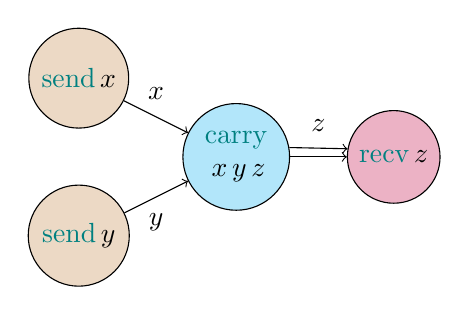
\begin{tikzpicture}[draw,circle]
    \node[draw,circle,fill opacity=0.3,text opacity=1,fill=brown] (send-x) at (0,2)   {$\func{send} \, x$};
    \node[draw,circle,fill opacity=0.3,text opacity=1,fill=brown] (send-y) at (0,0)   {$\func{send} \, y$};
    \node[draw,circle,fill opacity=0.3,text opacity=1,fill=purple] (recv-z) at (4,1)   {$\func{recv} \, z$};
    \node[draw,circle,fill opacity=0.3,text opacity=1,fill=cyan,align=center] (sync) at (2,1)   {$\func{carry}$\\$ \, x \, y \, z$};

    \draw[->] (send-x) -- node[above] {$x$} (sync);
    \draw[->] (send-y) -- node[below] {$y$} (sync);
    \draw[->] (sync.10) -- node[above] {$z$} (recv-z.170);
    \draw[->] (sync) -- (recv-z);
  \end{tikzpicture}
\end{center}

\todo{the colors are confusing: function color for send recv carry, individual colors for sender receiver and carrier}
Our courier system is defined by four \picalc{} processes composed in parallel instantiating the above three roles:
we have two \sender{} processes, $\func{send} \, x$ and $\func{send} \, y$, sending data over channels $x$ and $y$, respectively;
one \receiver{} process, $\func{recv} \, z$, which receives over channel $z$ the data sent from each of the senders -- hence receives twice;
and a \courier{} process $\func{carry} \, x \, y \, z$, which synchronises communication among the senders and the receiver.
The \courier{} process first receives data from the two senders along its input channels $x$ and $y$, and then sends the two received bits of data to the receiver along its output channel $z$.

The \sender{} and \receiver{} \emph{roles} are defined below, parametrised by the channels on which they operate.
The \sender{} creates a new channel to be sent as data, and sends it over channel $c$, and then terminates.
Each \sender{} process $\func{send} \, x$ and $\func{send} \, y$ is an instantiation of $\func{send} \, c$.
The \receiver{} receives data \emph{twice} on a channel $c$ and then terminates.
The \receiver{} process $\func{recv} \, z$ is an instantiation of $\func{recv} \, c$.
\todo{get rid of vertical space}
\begin{minipage}[t]{0.5\textwidth}
\begin{flalign*}
  & \func{send} \; : \; \Var_n \to \Process_n & \\
  & \func{send} \; c = \new{} \send{(\suc c)}{\constr{0}} \PO
\end{flalign*}
\end{minipage}
\begin{minipage}[t]{0.5\textwidth}
\begin{flalign*}
  & \func{recv} \; : \; \Var_n \to \Process_n & \\
  & \func{recv} \; c \; = \recv{c}{} \recv{(\suc c)} \PO
\end{flalign*}
\end{minipage}

The \courier{} role is defined below as $\func{carry} \; x \; y \; z$.
It sequentially receives on the two input channels $x$ and $y$ -- instantiating $in0$ and $in1$, and then outputs the two pieces of received data on the output channel $z$ -- instantiating $out$.
Finally, we create three communication channels and compose all four processes together: the first channel is shared between the one \sender{} and the \courier{}, the second between the other \sender{} and the \courier{}, and the third between the \receiver{}  and the \courier{}.
The result is the courier $\func{system}$ defined below.
\begin{minipage}[t]{0.5\textwidth}
\begin{flalign*}
  \func{carry} \; : \; \Var_n \to \Var_n \to \Var_n \to \Process_n%
\end{flalign*}%
\begin{flalign*}
  & \func{carry} \; in0 \; in1 \; out \; &&= \\
  & && \recv{in0 &&}{} \\
  & && \recv{(\suc \; in1) &&}{} \\
  & && \send{(\suc \suc \; out) &&}{\suc \constr{0}} \\
  & && \send{(\suc \suc \; out) &&}{\constr{0}} \PO
\end{flalign*}
\end{minipage}
\begin{minipage}[t]{0.5\textwidth}
\begin{flalign*}
  & \func{system} && : \; \Process_{\constr{0}} & \\
  & \func{system} && = \new{} ( \func{send} \; \constr{0} \\
  & && \comp{}{ \new{} ( \func{send} \; \constr{0} } \\
  & && \comp{}{ \new{} ( \func{recv} \; \constr{0} } \\
  & && \comp{}{ \func{carry} \; (\suc \suc \constr{0}) \; (\suc \constr{0}) \; \constr{0}))) } \\
\end{flalign*}
\end{minipage}
\todo{fix}

We continue this example and by providing typing derivations for these processes in \autoref{leftover-typing}.
There we use a mix of linear, graded and shared typing to type check $\func{system}$.
\end{example}

%%%%%%%%%%%%%%%%%%%%%%%%%%%%%%%%%%%%%%%%%%%%%%%%%%%%%%%%%%%%%%%%%%%
\section{Operational Semantics}
\label{semantics}
Thanks to our well-scoped grammar in \autoref{syntax}, the semantics of our language can now be defined on the totality of the syntax.
We define structural congruence in \autoref{structural-congruence} and provide a reduction relation in \autoref{operational-semantics}.

%%%%%%%%%%%%%%%%%%%%%%%%%%%%%%%%%%%%%%%%%%%%%%%%%%%%%%%%%%%%%%%%%%%
\subsection{Structural Congruence}
\label{structural-congruence}

\begin{nidefinition}
  \label{def:unused}
  We consider a variable $i$ to be unused in $P$ ($\Unused_i \; P$) if none of the inputs nor the outputs refer to it.
  $Unused_i \; P$ is defined as a recursive predicate on $P$, incrementing $i$ every time we go under a binder, and using $i \type{\not\equiv} x$ ( which unfolds to the negation of propositional equality on \textsc{Var}, i.e. $i \type{\equiv} x \to \type{\bot}$) to compare variables.
\end{nidefinition}

\begin{nidefinition}
We define the base cases of a structural congruence relation \textsc{StructCong} $\eqeq$ as follows:
\begin{mathpar}
  \datatype
  { }
  {P \eqeq Q : \Set}
  \; \textsc{StructCong}

  \inferrule
  { }
  {\constr{comp-assoc} : \comp{P}{(\comp{Q}{R})} \eqeq \comp{(\comp{P}{Q})}{R}}

  \inferrule
  { }
  {\constr{comp-sym} : \comp{P}{Q} \eqeq \comp{Q}{P}}
  
  \inferrule
  { }
  {\constr{comp-end} : \comp{P}{\PO_n} \eqeq P}
  
  \inferrule
  { }
  {\constr{scope-end} : \new \PO_{\suc n} \eqeq \PO_n}
  
  \inferrule
  {uQ : \Unused_{\constr{0}} \; Q}
  {\constr{scope-ext} : \new (\comp{P}{Q}) \eqeq \comp{(\new P)}{\func{lower}_{\constr{0}} \; \; Q \; uQ}}

  \inferrule
  { }
  {\constr{scope-comm} : \new \new P \eqeq \new \new \func{exchange}_{\constr{0}} \; P}
\end{mathpar}

The first three rules ($\constr{comp}-$*) state associativity, symmetry, and $\PO$ as being the neutral element of parallel composition, respectively.
The last three ($\constr{scope}-$*) state garbage collection, scope extrusion and commutativity of restrictions, respectively.
In $\constr{scope-ext}$ the side condition $\Unused_i \; Q$ makes sure that $i$ is unused in $Q$ (see \autoref{def:unused}).
The function $\func{lower}_i \; Q \; uQ$ traverses $Q$ decrementing every index greater than $i$.
In $\constr{scope-comm}$ the function $\func{exchange}_i \; P$ traverses $P$ (of type $\allowbreak \Process_{\suc \suc n}$) and swaps variable references $i$ and $\suc i$.
In all the above, $i$ is incremented every time we go under a binder.
\end{nidefinition}

\begin{nidefinition}
We lift the relation \textsc{StructCong} $\eqeq{}$ and close it under equivalence and congruence in \textsc{Equals} $\eq{}$.
The relation \textsc{Equals} is structurally congruent under a context $\mathcal{C}[\cdot]$ \cite{Sangio01} and is reflexive, symmetric and transitive. 
\end{nidefinition}


%%%%%%%%%%%%%%%%%%%%%%%%%%%%%%%%%%%%%%%%%%%%%%%%%%%%%%%%%%%%%%%%%%%
\subsection{Reduction Relation}
\label{operational-semantics}

The operational semantics of the \picalc{} is defined as a reduction relation \textsc{Reduces} $\reduce{c}$ indexed by the channel $c$ on which communication occurs.
We keep track of channel $c$ so we can state subject reduction (\autoref{app:type-safety}).
\begin{mathpar}
  \datatype
  {n : \N}
  {\Channel_n : \Set}
  \; \textsc{Channel}

  \inferrule
  { }
  {\constr{internal} : \Channel_n}

  \inferrule
  {i : \Var_n}
  {\constr{external} \; i : \Channel_n}

  \datatype
  {c : \Channel_n \\ P \; Q : \Process_n}
  {P \reduce{c} Q : \Set}
  \; \textsc{Reduces}

  \inferrule
  {i \; j : \Var_n \\ P : \Process_{\suc n} \\ Q : \Process_n}
  {\constr{comm} : \comp{\recv{i}{}P}{\send{i}{j}{Q}} \reduce{\constr{external} \; i} \comp{\func{lower}_{\constr{0}} \; (\subst{P}{\suc j}{\constr{0}}) \; uP'}{Q}}

  \inferrule
  {red : P \reduce{c} P'}
  {\constr{par} \; red : \comp{P}{Q} \reduce{c} \comp{P'}{Q}}

  \inferrule
  {red : P \reduce{c} Q}
  {\constr{res} \; red : \new P \reduce{\func{dec}\; c} \new Q}

  \inferrule
  {eq_1 : P \eq{} P' \\ red : P' \reduce{c} Q' \\ eq_2 : Q' \eq{} Q}
  {\constr{struct} \; eq \; red : P \reduce{c} Q}
\end{mathpar}

We distinguish between channels that are created inside of the process ($\constr{internal}$), and channels that are created outside ($\constr{external}\ i$), where $i$ is the index of the channel variable.
In rule $\constr{comm}$, parallel processes reduce when they communicate over a common channel with index ${i}$.
As a result of that communication, the continuation of the input process $P$ has all the references to its most immediate variable substituted with references to $\suc j$, the variable sent by the output process $\send{i}{j}{Q}$.
After this substitution, $\subst{P}{\suc j}{\constr{0}}$ is \emph{lowered} --- all variable references are decreased by one (we apply \autoref{lm:substitution-unused} to obtain a proof $\Unused_{\constr{0}} \; (\subst{P}{\suc j}{\constr{0}})$).
Reduction is closed under parallel composition (rule $\constr{par}$), restriction (rule $\constr{res}$) and structural congruence (rule $\constr{struct}$) 
--- notably, not under input nor output, as doing so would not preserve the sequencing of actions \cite{Sangio01}.
\todo{why do we not apply structural congruence on both sides?}

\begin{nilemma}
  \label{lm:substitution-unused}
  For every variables $i$ and $j$, if $i \type{\not\equiv} j$ then $\Unused_i \allowbreak (\subst{P}{j}{i})$.
\end{nilemma}
\begin{proof}
  By structural induction on \textsc{Process} and \textsc{Var}.
\end{proof}

Rule $\constr{res}$ uses $\func{dec}$ to decrement the index of channel $c$ as we wrap processes $P$ and $Q$ inside a binder.
It is defined as follows:
\begin{equation*}
  \begin{aligned}
    & \func{dec} : \Channel_(\suc n) && \to \Channel_n \\
    & \func{dec} \; \constr{internal}                 && \hookrightarrow \constr{internal} \\
    & \func{dec} \; (\constr{external} \; \constr{0}) && \hookrightarrow \constr{internal} \\
    & \func{dec} \; (\constr{external} \; (\suc n))   && \hookrightarrow \constr{external} \; n \\
  \end{aligned}
\end{equation*}
\todo{introduce function definition syntax, fix alignment}

%%%%%%%%%%%%%%%%%%%%%%%%%%%%%%%%%%%%%%%%%%%%%%%%%%%%%%%%%%%%%%%%%%%
\section{Resource-aware Type System}
\label{type-system}

In \autoref{multiplicities} we characterise a usage algebra for our type system.
It defines how resources are \emph{split} in parallel composition and \emph{consumed} in input and output.
We define typing and usage contexts in \autoref{contexts}.
We provide a type system for a resource-aware \picalc{} in \autoref{leftover-typing}.

\subsection{Multiplicities and Capabilities}
%%%%%%%%%%%%%%%%%%%%%%%%%%%%%%%%%%%%%%%%%%%%%%%%%%%%%%%%%%%%%%%%%%%
\label{multiplicities}

In the linear \picalc{} each channel has an input and an output \emph{capability}, and each capability has a given \emph{multiplicity} of 0 (exhausted) or 1 (available).
We generalise over this notion by defining an algebra for multiplicities that is satisfied by linear, graded and shared types alike.
We then use pairs of multiplicities as usage annotations for a channel's input and output capabilities.

\begin{nidefinition}[Usage algebra]
  A \emph{usage algebra} is a ternary relation $\op{x}{y}{z}$ that is \emph{partial} (as not any two multiplicities can be combined), \emph{deterministic} and \emph{cancellative} (to aid equational reasoning), \emph{associative} and \emph{commutative} (following directly from subject congruence for parallel composition), and in which the leftovers can be \emph{computed} (as to automatically update the usage context every time input and output occurs).
  It has a \emph{neutral element} $\zero$ that is absorbed on either side, and that is also \emph{minimal} (so that new resources cannot arbitrarily spring into life).
  It has an element $\one$ that is used to count inputs and outputs.
  Below we define such an algebra as a record $\Algebra_C$ on a carrier $C$.
  We use $\forall$ for universal quantification.
  The dependent product $\type{\exists}$ uses the value of its first argument in the type of its second.
  The type $\type{DEC} \; P$ is a witness of either $P$ or $P \to \type{\bot}$, where $\type{\bot}$ is the empty type with no constructors.
  \begin{equation*}
  \begin{aligned}
    &\zero                   &:{} &                 &        & C \\
    &\one                    &:{} &                 &        & C \\
    &\op{\_}{\_}{\_}         &:{} &                 &        & C \to C \to C \to \Set \\
    &\func{\cdot-compute^r}  &:{} &\forall x y       & \to \; & \type{DEC} \; (\type{\exists} z  \; (\op{x}{y}{z})) \\
    &\func{\cdot-unique}     &:{} &\forall x x' y z  & \to \; & \op{x'}{y}{z} \to \op{x}{y}{z} \to x' \equiv x \\
    &\func{\cdot-unique^l}   &:{} &\forall x y y' z  & \to \; & \op{x}{y'}{z} \to \op{x}{y}{z} \to y' \equiv y \\
    &\func{\cdot-min^l}      &:{} &\forall y z        & \to \; & \op{\zero}{y}{z} \to y \equiv \zero \\
    &\func{\cdot-id^l}       &:{} &\forall x         & \to \; & \op{x}{\zero}{x} \\
    &\func{\cdot-comm}       &:{} &\forall x y z     & \to \; & \op{x}{y}{z} \to \op{x}{z}{y} \\
    &\func{\cdot-assoc}      &:{} &\forall x y z u v & \to \; & \op{x}{y}{z} \to \op{y}{u}{v} \to \\
    &                        &    &                  &        & \type{\exists} w  \; (\op{x}{u}{w} \times \op{w}{v}{z})
  \end{aligned}
  \end{equation*}
\end{nidefinition}

We sketch the implementation of linear, graded and shared types as instances of our usage algebra below.
Their use in typing derivations is illustrated in \autoref{example-derivation} (Continued).
\begin{center}
\begin{tabular}{l | l | l}
  & carrier & operation \\
  \hline
  \textbf{linear} & \makecell[cl]{$\constr{0} \, : \, \type{Lin}$ \\ $\constr{1} \, : \, \type{Lin}$} & \makecell[cl]{$\op{\constr{0}}{\constr{0}}{\constr{0}}$ \\ $\op{\constr{1}}{\constr{1}}{\constr{0}}$ \\ $\op{\constr{1}}{\constr{0}}{\constr{1}}$} \\
  \hline
  \textbf{graded} & \makecell[cl]{$\constr{0} \, : \type{Gra}$ \\ $\suc \, : \type{Gra} \to \type{Gra}$} & \makecell[cl]{$\forall \, x \, y \, z$ \\ $\to x \, \type{\equiv} \, y \, \func{+} \, z$ \\ $\to \op{x}{y}{z}$} \\
  \hline
  \textbf{shared} & $\constr{\omega} \, : \, \type{Sha}$ & $\op{\constr{\omega}}{\constr{\omega}}{\constr{\omega}}$ \\
\end{tabular}
\end{center}

%%%%%%%%%%%%%%%%%%%%%%%%%%%%%%%%%%%%%%%%%%%%%%%%%%%%%%%%%%%%%%%%%%% 
\subsection{Typing Contexts}
\label{contexts}

We use indexed sets of usage algebras to allow several usage algebras to coexist in our type system with leftovers (\autoref{leftover-typing}).
\begin{nidefinition}[Indexed set of usage algebras]
  An \emph{indexed set of usage algebras} is a type $\Idx$ of indices that is nonempty ($\type{\exists IDX}$) together with an interpretation $\Usage$ of indices into types, and an interpretation $\type{ALGEBRAS}$ of indices into usage algebras of the corresponding type.
  \begin{equation*}
    \begin{aligned}
      &\Idx               &:{} &\Set \\
      &\type{\exists IDX} &:{} &\Idx \\
      &\Usage             &:{} &\Idx \to \Set \\
      &\type{ALGEBRAS}    &:{} &(idx : \Idx) \to \Algebra_{\Usage_{idx}}
    \end{aligned}
  \end{equation*}
\end{nidefinition}

\todo{definition captions reset textsc}
We keep typing contexts ($\PreCtx$) and usage contexts ($\Ctx$) separate.
The former are preserved throughout typing derivations; the latter are transformed as a result of input, output, and context splits.
\begin{nidefinition}[\textsc{Type} and \textsc{PreCtx}: types and typing contexts]
  A \emph{type} is either a unit type ($\unit$), a base type ($\base{n}$) or a channel type ($\channel{t}{x}$) (first two constructors below).
  \begin{mathpar}
    \datatype
    { }
    {\Type : \Set}
    \; \textsc{Type}
  
    \inferrule
    { }
    {\unit : \Type}

    \inferrule
    {n : \N}
    {\base{n} : \Type}
  
    \inferrule
    {t : \Type \\ \stacked{idx : \Idx \\\\ x : \Usage_{idx}^{\func{2}}}}
    {\channel{t}{x} : \Type}
  \end{mathpar}
  
  \begin{mathpar}
    \datatype
    {n : \N}
    {\PreCtx_n : \Set}
    \; \textsc{PreCtx}
  
    \inferrule
        { }
        {[] : \PreCtx_{\constr{0}}}
  
        \inferrule
            {\gamma : \PreCtx_n \\ t : \Type}
            {\gamma \comma t : \PreCtx_{\suc n}}
  \end{mathpar}

  The unit type $\unit$ serves as a proof of inhabitance for types.
  The base type $\base{n}$ uses natural numbers as placeholders for types (the host language can then interpret the former into the latter --- e.g., $0$ as booleans, $1$ as natural numbers) so that we avoid having to deal with universe polymorphism.
  The type $\channel{t}{x}$ of a channel determines what type ${t}$ of data and what usage annotations ${x}$ are sent over that channel.
  This channel notation aligns with $[t]\ \mathbf{chan}_{(i^{y},o^{z})}$, where $y,z$ are the multiplicities of input $i$ and output $o$ capabilities, respectively \cite{K07}.

  A \emph{typing context} (last two rules above) is a length-indexed list of types, and is either empty $[]$ or the result of appending a type $t$ to an existing context $\gamma$r
\end{nidefinition}


\begin{nidefinition}[\textsc{Ctx}: usage contexts]
  A \emph{usage context} is a context $\Ctx_{idxs}$ of pairs of usage annotations that is indexed by a length-indexed context of indices $\Idxs_n$.
  A usage context is either empty $[]$ or the result or appending a usage annotation $x$ to an existing context $\Gamma$.
  \begin{mathpar}
    \datatype
    {n : \N}
    {\Idxs_n : \Set}
    \; \textsc{Idxs}
  
    \inferrule
        { }
        {[] : \Idxs_{\constr{0}}}
  
    \inferrule
        {idxs : \Idxs_n \\ idx : \Idx}
        {idxs \comma idx : \Idxs_{\suc n}}
  
    \datatype
    {idxs : \Idxs_n}
    {\Ctx_{idxs} : \Set}
    \; \textsc{Ctx}
    
    \inferrule
        { }
        {[] : \Ctx_{[]}}
        
    \inferrule
        {\Gamma : \Ctx_{idxs} \\ x : \Usage_{idx} ^{\func{2}}}
        {\Gamma \comma x : \Ctx_{idxs \comma idx}}
  \end{mathpar}

  We use the notation $\type{C}^{\func{2}}$ to stand for a $\type{C} \constr{\times} \type{C}$ pair of input and output multiplicities, respectively.
  Henceforth, we use $\lz$ to denote the multiplicity pair $0 \comma 0$, $\li$ for the pair $1 \comma 0$, $\lo$ for $0 \comma 1$, and $\lio$ for $1 \comma 1$.
  This notation was originally used in the linear \picalc{} \cite{KPT96,Sangio01}.
\end{nidefinition}

%%%%%%%%%%%%%%%%%%%%%%%%%%%%%%%%%%%%%%%%%%%%%%%%%%%%%%%%%%%%%%%%%%% 
\subsection{Typing with Leftovers}
\label{leftover-typing}

We present a resource-aware type system for the \picalc{} based on \emph{leftover typing} \cite{Allais2018a}, a technique that, in addition to the usual typing context $\PreCtx_n$ and (input) usage context $\Ctx_{idxs}$, adds an extra \emph{(output) usage context} $\Ctx_{idxs}$ to the typing rules.
This output context contains the \emph{leftovers} (the unused multiplicities) of the process being typed.
These leftovers can then be used as input to another typing derivation.

Leftover typing inverts the information flow concerning usage annotations so that it is the typing derivations of subprocesses which determine how resources are allocated.
As a result, context split proofs are no longer necessary.
Leftover typing also allows \emph{framing} to be stated, and \emph{weakening} and \emph{strengthening} to acquire a more general form.

Our type system is composed of two typing judgments: one for variable references (\autoref{def:varref}) and one for processes (\autoref{def:types}).
Both judgments are indexed by a typing context $\gamma$, an input usage context $\Gamma$, and an output usage context $\Delta$ (the leftovers).

The \textbf{typing judgement for variables} $\contains{\gamma}{\Gamma}{i}{t}{y}{\Delta}$ asserts that ``index $i$ in typing context $\gamma$ is of type $t$, and subtracting $y$ at position $i$ from input usage context $\Gamma$ results in leftovers $\Delta$''.
The \textbf{typing judgement for processes} $\types{\gamma}{\Gamma}{P}{\Delta}$ asserts that ``process $P$ is well typed under typing context $\gamma$, usage input context $\Gamma$ and leftovers $\Delta$''.


\begin{nidefinition}[\textsc{VarRef}: typing variable references]
  \label{def:varref}

  The \textsc{VarRef} typing relation for variable references is presented below.
  \begin{mathpar}
    \mprset{sep=0.5em}
  
    \datatype{
      \gamma : \PreCtx_n \\
      i : \Var_n \\
      \stacked{
        t : \Type \\\\
        idx : \Idx \\\\
        y : \Usage_{idx}^{\func{2}}} \\
      \stacked{
        idxs : \Idxs_n \\\\
        \Gamma \; \Delta : \Ctx_{idxs}}}
    {\contains{\gamma}{\Gamma}{i}{t}{y}{\Delta} : \Set}
    \; \textsc{VarRef}
  
    \inferrule
    {\opsquared{x}{y}{z}}
    {\constr{0} : \contains{\gamma \comma t}{\Gamma \comma x}{\constr{0}}{t}{y}{\Gamma \comma z}}
    
    \inferrule
    {loc_i : \contains{\gamma}{\Gamma}{i}{t}{x}{\Delta}}
    {\suc \; loc_i : \contains{\gamma \comma t'}{\Gamma \comma x'}{\suc i}{t}{x}{\Delta \comma x'}}
  \end{mathpar}

  The base case $\constr{0}$ splits the usage annotation $x$ of type $\Usage_{idx}$ into $y$ and $z$ (the leftovers).
  Note that the remaining context $\Gamma$ is preserved unused as a leftover.
  This splitting $\opsquared{x}{y}{z}$ is as per the usage algebra provided by the developer for the index $idx$.
  We use the \emph{computability} of the monoidal relation to alleviate the user from the proof burden $\opsquared{x}{y}{z}$.
  The inductive case $\suc$ appends the type $t'$ to the typing context, and the usage annotation $x'$ to both the input and output usage contexts. 

  We lift the operation $\op{x}{y}{z}$ and its algebraic properties to an operation $\opsquared{(x_l \comma x_r)}{(y_l \comma y_r)}{(z_l \comma z_r)}$ on pairs of multiplicities and an operation $\opctx{\Gamma}{\Delta}{\Xi}$ on usage contexts with the same underlying context of indices.
\end{nidefinition}

\begin{example}[Variable reference]
  We type a variable reference $\suc \constr{0}$ with type $\channel{\unit}{\li}$ and usage $\li$.
  \begin{flalign*}
  & \func{egVar} \; : \; \contains{(\constr{[]} \comma \channel{\unit}{\li} \comma \unit)} {\constr{[]} \comma \lio \comma \lio)} {\suc \constr{0}} {\channel{\unit}{\li}} {\li} {(\constr{[]} \comma \lo \comma \lio)}\\
  & \func{egVar} \; = \; \suc \constr{0}
  \end{flalign*}
  We must show that the variable with index $\suc \constr{0}$ is of type $\channel{\unit}{\li}$ and has a usage annotation $\li$ in an environment with a typing context $(\constr{[]} \comma \channel{\unit}{\li} \comma \unit)$ and a usage context $(\constr{[]} \comma \lio \comma \lio)$.
  The \textsc{VarRef} constructors that we must use are completely determined by the variable index $\suc \; \constr{0}$ in the type.
  The constructor $\suc$ steps under the outermost variable in the context, preserving its usage annotation $\lio$ from input to output.
  The constructor $\constr{0}$ asserts that the next variable is of type $\channel{\unit}{\li}$, and that the usage annotation $\lio$ can be split such that $\op{\lio}{\li}{\lo}$ --- we use $\func{\cdot-compute^r}$ to automatically fulfill this proof obligation.
\end{example}

\begin{nidefinition}[\textsc{Types}: typing processes]
  \label{def:types}

  The \textsc{Types} typing relation for \picalc{} processes is presented below.
  For convenience, we reuse the constructor names introduced for the syntax in \autoref{syntax}.
  \begin{mathpar}
    \datatype{
      \gamma : \PreCtx_n \\
      P : \Process_n \\
      \stacked{
        idxs : \Idxs_n \\\\
        \Gamma \; \Delta : \Ctx_{idxs}}}
    {\types{\gamma}{\Gamma}{P}{\Delta} : \Set}
    \; \textsc{Types}
    
    \inferrule
    { }
    {\PO : \types{\gamma}{\Gamma}{\PO}{\Gamma}}
  
    \inferrule
    {t : \Type \\ x : \Usage_{idx}^{\func{2}} \\ y : \Usage_{idx'} \\\\
     cont : \types{\gamma \comma \channel{t}{x}}{\Gamma \comma (y \comma y) }{P}{\Delta \comma \lz}}
    {\new \; t \; x \; y \; cont : \types{\gamma}{\Gamma}{\new P}{\Delta}}
  
    \inferrule
        {\stacked{
            chan_i : \contains{\gamma \hspace{1.0em}}{\Gamma \hspace{1.0em}}{i}{\channel{t}{x}}{\li}{\Xi} \\\\
            cont \hspace{0.5em} : \types{\gamma \comma t}{\Xi \comma x}{P \hspace{4.2em}}{\Theta \comma \lz}}}
        {\recv{chan_i}{} cont : \types{\gamma}{\Gamma}{\recv{i}{}P}{\Theta}}
  
    \inferrule
        {\stacked{
            chan_i : \contains{\gamma}{\Gamma \hspace{0.1em}}{i}{\channel{t}{x}}{\lo}{\Delta} \\\\
            loc_j \hspace{0.7em} : \contains{\gamma}{\Delta}{j}{t \hspace{2.8em}}{x \hspace{0.2em}}{\Xi} \\\\
            cont \hspace{0.5em} : \types{\gamma}{\Xi}{\hspace{0.4em}P\hspace{4.0em}}{\Theta}}}
        {\send{chan_i}{loc_j} cont : \types{\gamma}{\Gamma}{\send{i}{j}P}{\Theta}}
  
    \inferrule
    {l : \types{\gamma}{\Gamma}{P\hspace{0.3em}}{\Delta} \\\\
     r : \types{\gamma}{\Delta}{Q}{\Xi}}
    {\comp{l}{r} : \types{\gamma}{\Gamma}{\comp{P}{Q}}{\Xi}}
  \end{mathpar}

  The inaction process in rule $\PO$ does not change usage annotations.
  The scope restriction in rule $\new$ expects three arguments: the type $t$ of data being transmitted; the usage annotation $x$ of what is being transmitted; and the multiplicity $y$ given to the channel itself.
  This multiplicity $y$ is used for both input and output, so that they are balanced.
  The continuation process $P$ is provided with the new channel with usage annotation $y \comma y$, which it must completely exhaust.
%
  The input process in rule $\recv{}{}$ requires a channel $chan_i$ at index $i$ with usage $\li$ available, such that data with type $t$ and usage $x$ can be sent over it.
  Note that the index $i$ is used in the syntax of the typed process.
  We use the leftovers $\Xi$ to type the continuation process, which is also provided with the received element --- of type $t$ and multiplicity $x$ --- at index $\constr{0}$.
  The received element $x$ must be completely exhausted by the continuation process.
%
  Similarly to input, the output process in rule $\send{}{}$ requires a channel $chan_i$ at index $i$ with usage $\lo$ available, such that data with type $t$ and usage $x$ can be sent over it.
  We use the leftover context $\Delta$ to type the transmitted data, which needs an element $loc_j$ at index $j$ with type $t$ and usage $x$, as per the type of the channel $chan_i$.
  The leftovers $\Xi$ are used to type the continuation process.
  Note that both indices $i$ and $j$ are used in the syntax of the typed process.
%
  Parallel composition in rule $\comp{}{}$ uses the leftovers of the left-hand process to type the right-hand process.
  By keeping track in the typing derivation of $P$ of the resources $P$ uses, we can use them to type $Q$ and save the user from having to provide a top-down proof of context split.
\end{nidefinition}

\begin{example}[Typing derivation, continues=example-process]
\label{example-derivation}

We provide the typing derivation for the courier system defined in \autoref{example-process}.
For the sake of simplicity, we instantiate these processes with concrete variable references before typing them.

The \receiver{} defined by the $\func{recv}$ process receives data along the channel with index $0$, thus that variable needs to be of channel type $\channel{t}{u}$ for some $t$ and $u$.
After receiving twice, the process ends, and we should not be left with any unused multiplicities: $u$ needs to be $\lz$.
We will use graded types to keep track of the exact number of times communication happens.
Whatever the input multiplicity of the channel, we will consume $2$ of it and leave the remaining as leftovers.
Once the types are given, the typing derivation is completely syntax directed.
\begin{multicols}{2}
\begin{flalign*}
  & \func{\vdash recv} \; && : \; \types{\gamma \comma \channel{t}{\lz}\\ & &&}{\Gamma \comma (\suc \suc l \comma r)\\ & &&}{\func{recv} \; \constr{0}\\ & &&}{\Gamma \comma (l \comma r)} & \\
  & \func{\vdash recv} \; && = \; \recv{\constr{0}}{} \recv{(\suc \constr{0})}{} \PO
\end{flalign*}
\begin{flalign*}
  & \func{\vdash send} \; && : \; \types{\gamma \comma \channel{\channel{\unit}{\func{\omega}}}{\lz}\\ & &&}{\Gamma \comma (l \comma \suc r)\\ & &&}{\func{send} \; \constr{0}\\ & &&}{\Gamma \comma (l \comma r)} & \\
  & \func{\vdash send} \; && = \; \new{} \; \_ \; \_ \; \zero \; \send{(\suc \constr{0})}{\constr{0}} \PO
\end{flalign*}
\end{multicols}

The \sender{} defined by the $\func{send}$ process sends data along the channel with index $0$, thus that variable needs to be of channel type $\channel{t}{u}$ for some $t$ and $u$.
We instantiate $t$ (the type of data that the \sender{} sends) to $\channel{\unit}{\func{\omega}}$, as that is a value we can easily construct.
As per the type of the process $\func{recv}$, the transmitted multiplicities $u$ are $\lz$.
We will transmit once, thus use a single output multiplicity, and leave the rest as leftovers.
Agda can uniquely determine the arguments required by the $\new{}$ constructor, and thus we can omit them using underscores.

Dually, the \courier{} defined by the $\func{carry}$ process expects input multiplicities for the channels shared with $\func{send}$ and output multiplicities for the channel shared with $\func{recv}$.
The typing derivation here is uniquely determined by the type and syntax of the process.
\begin{multicols}{2}
\begin{flalign*}
& \func{\vdash carry} && : \types{\gamma \comma \channel{t}{\lz} \comma \channel{t}{\lz} \comma \channel{t}{\lz}\\ & &&}{\Gamma \comma (\suc lx \comma rx) \comma (\suc ly \comma ry) \comma (lz \comma \suc \suc rz)\\ & &&}{\func{carry} \; (\suc \suc \constr{0}) \; (\suc \constr{0}) \; \constr{0}\\ & &&}{\Gamma \comma (lx \comma rx) \comma (ly \comma ry) \comma (lz \comma rz)} & \\
& \func{\vdash carry} && = \\
& && \recv{(\suc \suc \constr{0})}{} \\
& && \recv{(\suc \suc \constr{0})}{} \\
& && \send{(\suc \suc \constr{0})}{\suc \constr{0}} \\
& && \send{(\suc \suc \constr{0})}{\constr{0}} \PO
\end{flalign*}
\begin{flalign*}
& \func{\vdash system} && : \; \types{\constr{[]}}{\constr{[]}}{\func{system}}{\constr{[]}} & \\
& \func{\vdash system} && = \new{} \; \_ \; \_ \; \_ \; ( \func{\vdash send} \\
& && \comp{}{ \new{} \; \_ \; \_ \; \_ } \; ( \func{\vdash send} \\
& && \comp{}{ \new{} \; \_ \; \_ \; \_ } \; ( \func{\vdash recv} \\
& && \comp{}{ \func{\vdash carry} })))
\end{flalign*}
\end{multicols}

We can now compose these processes in parallel and type the courier system.
Specifying the types of the channels is not required: Agda can infer them from the types of the processes.
\end{example}

%%%%%%%%%%%%%%%%%%%%%%%%%%%%%%%%%%%%%%%%%%%%%%%%%%%%%%%%%%%%%%%%%%% 
\section{Meta-Theory} \label{meta-theory}

We have mechanised subject reduction for our \picalc{} with leftovers in 850 lines of Agda code.
The meta-theory of resource-aware type systems often needs to reason on typing derivations modulo associativity in the allocation of resources.
For type systems using context splitting side conditions, this means applying associativity lemmas to recompute context splits; for type systems using leftover typing, this comes naturally \todo{rephrase?}.
An example use of this is showing that the application of $\constr{comp-asssoc}$ preserves typing: the proof proceeds by deconstructing the input derivation into $\comp{P}{(\comp{Q}{R})}$ and reassembling it as $\comp{(\comp{P}{Q})}{R}$ without the need of any extra reasoning.

All the reasoning carried out in our type safety proofs is based on the algebraic properties introduced in \autoref{multiplicities} -- an exception to this is $\func{\cdot -compute^r}$, which is only ever used for the user's convenience.
This algebraic properties of the algebras allow us to see a typing derivation $\types{\gamma}{\Gamma}{P}{\Delta}$ as a unique \emph{arrow} from $\Gamma$ to $\Delta$, and to freely compose arrows with the same typing context and a matching output and input usage contexts.

Leftover typing also allows us to prove a \emph{framing} theorem, which states that arbitrary usage annotations can be added to the input usage context, as long as they are added to the output usage context as well -- one can thus understand a typing derivation independently from its unused resources.
An example use of this is showing that $\constr{comp-comm}$ preserves typing: we use framing to show that in $\comp{P}{Q}$ the typing of $P$ and $Q$ is independent of one another.
\begin{nitheorem}[Framing]
  \label{thm:framing}
  Let $P$ be well typed in $\types{\gamma}{\Gamma_l}{P}{\Xi_l}$.
  Let $\Delta$ be such that $\opctx{\Gamma_l}{\Delta}{\Xi_l}$.
  Let $\Gamma_r$ and $\Xi_r$ be arbitrary contexts such that $\opctx{\Gamma_r}{\Delta}{\Xi_r}$.
  Then $\types{\gamma}{\Gamma_r}{P}{\Xi_r}$.
\end{nitheorem}

Leftover typing allows \emph{weakening} and \emph{strengthening} to acquire a more general form, in which variables can freely be added or removed from context regardless of their usage annotation -- as long as this usage annotation is added or removed from the leftover context as well.
Weakening states that inserting a new variable into the context preserves the well-typedness of a process as long as the usage annotation of the inserted variable is preserved as a leftover.
Strengthening states that removing an unused variable preserves the well-typedness of a process.

\begin{nitheorem}[Weakening]
  \label{thm:weakening}
  Let $\func{ins}_i$ insert an element into a context at position $i$ --- for simplicity, we use it both to insert types into typing contexts and usage annotations into usage contexts.
  Let $P$ be well typed in $\types{\gamma}{\Gamma}{P}{\Xi}$.
  Then, lifting every variable greater than or equal to $i$ in $P$ is well typed in
  $\types{\func{ins}_i \; t \; \gamma}{\func{ins}_i \; x \; \Gamma}{\func{lift}_i \; P}{\func{ins}_i \; x \; \Xi}$.
\end{nitheorem}

\begin{nitheorem}[Strengthening]
  \label{thm:strengthening} 
  Let $\func{del}_i$ delete the element at position $i$ from a context --- for simplicity, we use it both to delete types from typing contexts and usage annotations from usage contexts.
  Let $P$ be well typed in $\types{\gamma}{\Gamma}{P}{\Xi}$.
  Let $i$ be a variable not in $P$, such that $uP \; : \; \Unused_i \; P$.
  Then lowering every variable greater than $i$ in $P$ is well typed in $\types{\func{del}_i \; \gamma}{\func{del}_i \; \Gamma}{\func{lower}_i \; P \; uP}{\func{del}_i \; \Xi}$.
\end{nitheorem}

\subsubsection{Type Safety}
Subject congruence states that applying structural congruence (\autoref{structural-congruence}) to a well-typed process preserves its well-typedness.
Subject reduction states that a well-typed process that communicates on a channel $c$ (\autoref{operational-semantics}) preserves its well-typedness and consumes $\lio$ from $c$ if $c$ is a channel in the environment.

\begin{nitheorem}[Subject congruence]
  \label{thm:subject-congruence}
  If $P \eq{} Q$ and $\types{\gamma}{\Gamma}{P}{\Xi}$, then $\types{\gamma}{\Gamma}{Q}{\Xi}$.
\end{nitheorem}

\begin{nitheorem}[Subject reduction]
  \label{thm:subject-reduction}
  Let $P$ be well typed in $\types{\gamma}{\Gamma}{P}{\Xi}$ and reduce such that $P \reduce{c} Q$.
  \begin{itemize}
    \item If $c$ is $\constr{internal}$, then $\types{\gamma}{\Gamma}{Q}{\Xi}$.
    \item If $c$ is $\constr{external} \; i$ and $\containsusage{\Gamma}{i}{\lio}{\Delta}$, then $\types{\gamma}{\Delta}{Q}{\Xi}$.
  \end{itemize}
\end{nitheorem}

We refer to \autoref{app:type-safety} \todo{autoref} for a more detailed account of the mechanised type-safety proofs.

%%%%%%%%%%%%%%%%%%%%%%%%%%%%%%%%%%%%%%%%%%%%%%%%%%%%%%%%%%%%%%%%%%% 
\section{Related Work}

\paragraph*{Extrinsic Encodings}

Extrinsic encodings define a syntax (often well-scoped) and a runtime semantics prior to any type system.
This allows one to talk about ill-typed terms, and defers the proof of subject reduction to a later stage.

To the best of our knowledge, leftover typing makes its appearance in 1994, when Ian Mackie first uses it to formulate intuitionistic linear logic \cite{Mackie}.
Allais \cite{Allais2018a} uses leftover typing to mechanise in Agda a bidirectional type system for the linear \lambdacalc{}.
He proves type preservation and provides a decision procedure for type checking and type inference.
In this paper, we follow Allais \cite{Allais2018a} and apply leftover typing to the \picalc{} for the first time.
We generalise the usage algebra, leading to linear, graded and shared type systems.
Drawing from quantitative type theory (by McBride and Atkey \cite{McBride2016,Atkey2018}), in our work we too are able to talk about fully consumed resources --- e.g., we can transmit $\lz$ multiplicities of a fully exhausted channel.

Recent years have seen an increase in the efforts to mechanise resource-aware process algebras, but one of the earliest works is the mechanisation of the linear \picalc{} in Isabelle/HOL by Gay \cite{Gay2001}.
Gay encodes the \picalc{} with linear and shared types using de Bruijn indices, a reduction relation and a type system posterior to the syntax.
However, in his work typing rules demand user-provided context splits, and variables with consumed usage annotations are erased from context.
We remove the demand for context splits, preserve the ability to talk about consumed resources, and adopt a more general usage algebra.

Orchard et al. introduce Granule \cite{Orchard}, a fully-fledged functional language with graded modal types, linear types, indexed types and polymorphism.
Modalities include exact usages, security levels and intervals; resource algebras are pre-ordered semirings with partial addition.
The authors provide bidirectional typing rules, and show the type safety of their semantics.

The work by Goto et al. \cite{Goto2016a} is, to the best of our knowledge, the first formalisation of session types which comes along with a mechanised proof of type safety in Coq.
The authors extend session types with polymorphism and pattern matching.
They use a locally-nameless encoding for variable references, a syntax prior to types, and an LTS semantics that encodes session-typed processes into the \picalc{}.
Their type system uses reordering of contexts and extrinsic context splits, which are not needed in our work. 

\paragraph*{Intrinsic Encodings}
 
Intrinsic encodings merge syntax and type system.
As a result, one can only ever talk about well-typed terms, and the reduction relation by construction carries a proof of subject reduction.
Significantly, by merging the syntax and static semantics of the object language one can fully use the expressive power of the host language.

Thiemann formalises in Agda the MicroSession (minimal GV \cite{Gay2010}) calculus with support for recursion and subtyping \cite{Thiemann2019}.
As Gay does in \cite{Gay2001}, context splits are given extrinsically, and exhausted resources are removed from typing contexts altogether.
The runtime semantics are given as an intrinsically typed CEK machine with a global context of session-typed channels.

In their recent paper, Ciccone and Padovani mechanise a dependently-typed linear \picalc{} in Agda \cite{Ciccone}.
Their intrinsic encoding allows them to leverage Agda's dependent types to provide a dependently-typed interpretation of messages --- to avoid linearity violations the interpretation of channel types is erased.
Message input is modeled as a dependent function in Agda, and as a result message predicates, branching, and variable-length conversations can be encoded.
In contrast to our work, their algebra is on the multiplicities $0$, $1$, $\omega$, and top-down context splitting proofs must be provided.

In another recent work, Rouvoet et al. provide an intrinsic type system for a \lambdacalc{} with session types \cite{Rouvoet2020}.
They use proof relevant separation logic and a notion of a supply and demand \emph{market} to make context splits transparent to the user.
Their separation logic is based on a partial commutative monoid that need not be deterministic nor cancellative.
Their typing rules preserve the balance between supply and demand, and are extremely elegant.
They distill their typing rules even further by modelling the supply and demand market as a state monad.

\paragraph*{Other Work}

Castro et al. \cite{Castro2020} provide tooling for locally-nameless representations of process calculi in Coq, where de Bruijn indices are not as popular as in Agda or Idris.
As a use-case, they use their tool to help automate proofs of subject reduction for a type system with session types.

Orchard and Yoshida \cite{OrchardY16} embed a small effectul imperative language into the session-typed \picalc{}, showing that session types are expressive enough to encode effect systems.

Based on contextual type theory \cite{Pientkaa,Pientka}, LINCX \cite{Georges2017} extends the linear logical framework LLF \cite{Cervesato1996} by internalising the notion of bindings and contexts.
The result is a meta-theory in which HOAS encodings with both linear and dependent types can be described.
The developer obtains for free an equational theory of substitution and decidable typechecking without having to encode context splits within the object language.

Further work on mechanising the \picalc{} \cite{Henry-Gerard1999,Honsell2001a,Bengtson2013,Despeyroux2000,Affeldt2008}, focuses on non-linear variations, whereas we present a range of linear, graded and shared types.

%%%%%%%%%%%%%%%%%%%%%%%%%%%%%%%%%%%%%%%%%%%%%%%%%%%%%%%%%%%%%%%%%%% 
\section{Conclusion and Future Work}

In this paper we provide a well-scoped syntax and a semantics for the \picalc{}, extrinsically define a type system on top of the syntax capable of handling linear, graded and shared types under the same unified framework and show that reduction preserves the well-typedness of processes.
We avoid the need for extrinsic context splits by defining a type system based on leftover typing \cite{Allais2018a}, which is defined here for the first time for the \picalc{}.
As a result, theorems like framing, weakening and strengthening can now be stated for the linear \picalc{}.
Our work is fully mechanised in around 1850 lines of code in Agda \cite{Zalakain2020Agda}.

As future work, we intend to prove further properties of our type system, such as that reduction preserves the balancing of channels.
We intend to add support for products, sum types and replication to both our syntax and our type system.
Orthogonally, making our typing rules bidirectional would allow us to provide a decision procedure for type checking processes in a given set of algebras.
Furthermore, it might also be worth identifying correspondences between our usage algebra and particular state machines.
Finally, we will use our \picalc{} with leftovers as an underlying framework on top of which we can implement session types and other advanced type theories.

\subsection{Replication}
\label{replication}

Replication can be added to a resource-algebra-agnostic type system with the following rule:
\begin{mathpar}
  \inferrule
  {\types{\gamma}{\Gamma}{P}{\Gamma}}
  {\types{\gamma}{\Gamma}{!P}{\Gamma}}
\end{mathpar}
That is, if a process consumes no resources (e.g. they are shared), then the process can be executed infinitely many times.
To show subject congruence, one has to prove that $P \eqeq \comp{P}{!P}$ preserves types in both directions.
In our setting, that means showing that $\types{\gamma}{\Gamma}{\comp{P}{!P}}{\Delta}$ then $\types{\gamma}{\Gamma}{!P}{\Delta}$.
Eliminating the hypothesis gives $\types{\gamma}{\Gamma}{P}{\Xi}$ and $\types{\gamma}{\Xi}{!P}{\Delta}$, eliminating the latter unifies $\Xi$ and $\Delta$ resulting in $\types{\gamma}{\Xi}{P}{\Xi}$.
To satisfy the goal $\types{\gamma}{\Gamma}{!P}{\Xi}$, one has to show that $\Gamma$ and $\Xi$ are equivalent too.
Note that the process $P$ does not syntactically restrict the types of the channels created within $P$.
That means that within the typing derivations $\types{\gamma}{\Gamma}{P}{\Xi}$ and $\types{\gamma}{\Xi}{P}{\Xi}$ one can create channels that transmit different amounts of data in $\Gamma$ and in $\Xi$, which are then not necessarily the same anymore.

%%%%%%%%%%%%%%%%%%%%%%%%%%%%%%%%%%%%%%%%%%%%%%%%%%%%%%%%%%%%%%%%%%% 
\section*{Acknowledgments}

We further want to thank Erika Kreuter, Wen Kokke, James Wood, Guillaume Allais, Bob Atkey, and Conor McBride for their work and thoughts.

\bibliographystyle{splncs04}
\bibliography{paper}

%%
\appendix
%% Appendix
\section{Structural Congruence}
\label{app:struct}

Structural congruence is a congruent equivalence relation.
As such, rewrites can happen anywhere inside a process, and are closed under reflexivity, symmetry and transitivity as shown by the first row of \autoref{fig:struct-cong1}.
The rest of the rules defines structural congruence under a context $\mathcal{C}[\cdot]$ \cite{Sangio01}, respectively restriction, composition, input and output.

\begin{figure}[h]
  \begin{mathpar}
    \datatype
    { }
    {\Rec : \Set}
    \; \textsc{Rec}
  
    \inferrule
    { }
    {\constr{zero} : \Rec}
    
    \inferrule
    {r : \Rec}
    {\constr{one} \; r : \Rec}
  
    \inferrule
    {r \; s : \Rec}
    {\constr{two} \; r \; s : \Rec}
    
    \datatype
    {P \, Q : \Process_n \\ r : \Rec}
    {P \eq{r} Q : \Set}
    \; \textsc{Equals}
  
    \inferrule
    {eq : P \eqeq Q}
    {\constr{struct} \; eq : P \eq{\constr{zero}} Q}
  
    \inferrule
    {eq : P \eq{r} P'}
    {\constr{cong-scope} \; eq : \new P \eq{\constr{one} \; r} \new P'}
  
    \inferrule
    {eq : P \eq{r} P'}
    {\constr{cong-comp} \; eq : \comp{P}{Q} \eq{\constr{one} \; r} \comp{P'}{Q}}
  
    \inferrule
    {eq : P \eq{r} P'}
    {\constr{cong-recv} \; eq : \recv{x}P \eq{\constr{one} \; r} \recv{x}P'}
  
    \inferrule
    {eq : P \eq{r} P'}
    {\constr{cong-send} \; eq : \send{x}{y}P \eq{\constr{one} \; r} \send{x}{y}P'}
  
    \inferrule
    { }
    {\constr{refl} : P \eq{\constr{zero}} P}
  
    \inferrule
    {eq : P \eq{r} Q}
    {\constr{sym} \; eq : Q \eq{\constr{one} \; r} P}
  
    \inferrule
    {eq_1 : P \eq{r} Q \\ \; eq_2 : Q \eq{s} R}
    {\constr{trans} \; eq_1 \; eq_2 : P \eq{\constr{two} \; r \; s} R}
  \end{mathpar}
  \caption{Structural rewriting rules lifted to a congruent equivalence relation indexed by a recursion tree.}
  \label{fig:struct-cong1}
  \end{figure}

In the transitivity rule, we must show that if $P$ is structurally congruent to $Q$ and $Q$ is to $R$, and $P$ is well-typed, then so is $R$.
To do so, we need to proceed by induction and first get a proof of the well-typedness of $Q$, then use that to reach $R$.
To show the typechecker that the doubly recursive call terminates we index the equivalence relation $=$ by a type $\Rec$ that models the structure of the recursion.

\section{Usage Algebra}
\label{app:usage-algebra}

\todo{we haven't introduced the forall and implicit syntax}
\todo{introduce DEC and exists}

Our usage algebra is a ternary relation $\op{x}{y}{z}$ that is \emph{partial}, \emph{functional}, \emph{cancelative}, \emph{associtive}, and \emph{commutative}.
It has a \emph{neutral element} $\zero$ that is absorbed on either side, and that is also \emph{minimal}.
It has an element $\one$ that is used to count inputs and outputs.
These algebraic laws are defined as a record $\Quantifier_C$ on a carrier set $C$ in \autoref{fig:multiplicities}.
We use a terniary relation to model the partial monoidal operation.

\begin{figure}[h]
\begin{equation}
\begin{aligned}
  &\zero                  &:{} &                      &        & C \\
  &\one                   &:{} &                      &        & C \\
  &\op{\_}{\_}{\_}        &:{} &                      &        & C \to C \to C \to et \\
  &\field{\cdot-compute}  &:{} &\forall y z           & \to \; & \type{DEC} \; (\type{\exists} x . \; (\op{x}{y}{z})) \\
  &\field{\cdot-unique}   &:{} &\forall \{x x' y z\}  & \to \; & \op{x'}{y}{z} \to \op{x}{y}{z} \to x' \equiv x \\
  &\field{\cdot-unique^l} &:{} &\forall \{x y y' z\}  & \to \; & \op{x}{y'}{z} \to \op{x}{y}{z} \to y' \equiv y \\
  &\field{0\cdot-min^l}   &:{} &\forall \{y z\}       & \to \; & \op{\zero}{y}{z} \to y \equiv \zero \\
  &\field{\cdot-id^l}     &:{} &\forall \{x\}         & \to \; & \op{x}{\zero}{x} \\
  &\field{\cdot-comm}     &:{} &\forall \{x y z\}     & \to \; & \op{x}{y}{z} \to \op{x}{z}{y} \\
  &\field{\cdot-assoc}    &:{} &\forall \{x y z u v\} & \to \; & \op{x}{y}{z} \to \op{y}{u}{v} \to \type{\exists} w . \; (\op{x}{u}{w} \times \op{w}{v}{z})
\end{aligned}
\end{equation}
\caption{Quantifier algebra $\Quantifier_C$ algebra on a partial commutative monoid.}
\label{fig:multiplicities}
\end{figure}

\section{Indexed Set of Usage Algebras}
\label{app:indexed-set-usage-algebra}

\begin{figure}[h]
  \begin{equation}
    \begin{split}
      &\field{IDX}          &:{} &\Set \\
      &\field{\exists IDX}  &:{} &\field{IDX} \\
      &\field{CARRIER}      &:{} &\field{IDX} \to \Set \\
      &\field{QUANTIFIERS}  &:{} &(i : \field{IDX}) \to \Quantifier_{\field{CARRIER}_i}
    \end{split}
  \end{equation}
  \caption{Indexed set of usage algebras.}
  \label{fig:indexed-multiplicities}
\end{figure}

\section{Lemmas for Type Safety}
\label{app:lemmas-type-safety}

\begin{nilemma}
  \label{lm:lower-lift}
  The function $lower_i \; P \; uP$ has an inverse $lift_i \; P$ that increments every $\textsc{Var}$ greater than or equal to $i$, such that $lift_i \; (lower_i \; P \; uP) \equiv P$.
\end{nilemma}
\begin{proof}
  By structural induction on \textsc{Process} and \textsc{Var}.
\end{proof}

\begin{nilemma}
  \label{lm:swap-swap}
  The function $swap_i \; P$ is its own inverse: $swap_i \; (swap_i \; P) \equiv P$.
\end{nilemma}
\begin{proof}
  By structural induction on \textsc{Process} and \textsc{Var}.
\end{proof}


\end{document}
